%##################################################
% FoF
%##################################################
\section{Friends-of-Friends algorithm}
\bartchapterimage{heic1006a_small.jpg}
\bartthumb{thumbs/heic1006a.png}
\begin{frame}

    \frametitle{Friends-of-Friends algorithm}

    \begin{columns}
        \begin{column}{0.65\textwidth}
        \end{column}
        \begin{column}{0.35\textwidth}
            \only<1>{%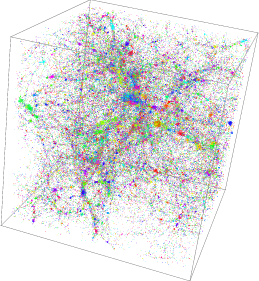
\includegraphics[width=\textwidth]{cubemock.png}}
            }
            \only<2>{%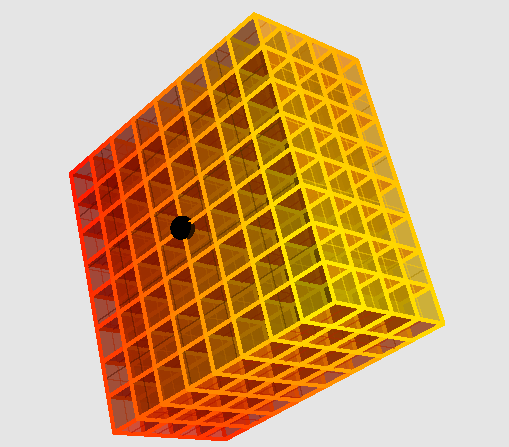
\includegraphics[width=\textwidth]{mock.pdf}}
            }
        \end{column}
    \end{columns}
\end{frame}

\begin{frame}
    \begin{tikzpicture}[scale=0.4]
        \tikzstyle{dots}=[draw, shape=circle, fill=black, text=white,
        scale=0.5]
        \tikzstyle{searched}=[line width=1.5pt, blue!90!white]
        \tikzstyle{linked}=[line width=2pt]
        \node[dots] (1) at (0, 1) {1};
        \node[dots] (2) at (1, 2) {2};
        \node[dots] (3) at (3, 4) {3};
        \node[dots] (4) at (4, 7) {4};
        \node[dots] (5) at (3, 6) {5};
        \node[dots] (6) at (8, 4) {6};
        \node[dots] (7) at (7, 3) {7};
        \node[dots] (8) at (10, 1) {8};

        \draw[searched, visible on=<2>] (1) circle (3);
        \draw[<->, blue, line width=1pt, visible on=<2>] (1.center) --
        ([shift=(1.center)]-30:3) node[right] {$b$};

        \draw[linked, green, visible on=<3->] (1) -- (2);
        \node[dots, fill=green, text=black, visible on=<3->] (1) at (0, 1)
            {1};
        \node[dots, fill=green, text=black, visible on=<3->] (2) at (1, 2)
            {2};

        \draw[searched, visible on=<4>] (2) circle (3);

        \draw[linked, green, visible on=<5->] (2) -- (3);
        \node[dots, fill=green, text=black, visible on=<5->] (3) at (3, 4)
            {3};

        \draw[searched, visible on=<6>] (3) circle (3);

        \draw[linked, green, visible on=<7->] (3) -- (5);
        \node[dots, fill=green, text=black, visible on=<7->] (5) at (3, 6)
            {5};

        \draw[searched, visible on=<8>] (5) circle (3);

        \draw[linked, green, visible on=<9->] (4) -- (5);
        \node[dots, fill=green, text=black, visible on=<9->] (4) at (4, 7)
            {4};

        \draw[searched, visible on=<10>] (6) circle (3);

        \draw[linked, purple, visible on=<10->] (6) -- (7);
        \node[dots, fill=purple, text=black, visible on=<10->] (6) at (8, 4)
            {6};
        \node[dots, fill=purple, text=black, visible on=<10->] (7) at (7, 3)
            {7};

        \draw[searched, visible on=<11>] (7) circle (3);

        \node[dots, fill=orange, text=black, visible on=<12>] (8) at (10, 1)
            {8};
    \end{tikzpicture}
\end{frame}
